\documentclass[fleqn]{article}
\usepackage{brochure-venturis}
\def\wLaTeX{L\kern-.25em\raisebox{.5ex}{\fontsize{70}{0}\selectfont
    \textsc{a}}\kern-.12em T\kern-0.1667em\raisebox{-.5ex}{E}\kern-.1em X}
\begin{document}
\noindent\begin{tabular}{
  @{}%	                   flush left margin
  b{.35\columnwidth}%	   logo
  @{\hspace{.03\columnwidth}}%        gap
  >{\huge\centering\color{DarkBlue}}p{.62\columnwidth}%	   headline
  @{}%                     flush right margin
}
  \raisebox{-55pt}{%
    
\includegraphics[width=.37\columnwidth]{images/logo.jpeg}
    }
&
     University of Victoria\linebreak
     Horticulture Club\par\vspace{8pt}\hrule height3pt
  \par\bigskip
  \fontsize{16}{18}\selectfont\itshape
  March 2023 Newsletter\linebreak
\end{tabular}

\noindent\begin{tabular}{@{}
                         p{.38\columnwidth}%		blurb
		         @{\hspace{.04\columnwidth}}% 	gap
		         p{.58\columnwidth}%		quotes
		         @{}%			implicit margin
}

% Left Column
\sffamily\lite\fontsize{16}{18}\selectfont\raggedright 
A tour of the greenhouse led by Dr. Patrick von Aderkas, and\linebreak\
a social plant swap in the Student Union Building with lots of free propagules!
\par\bigskip

\small\rightskip=0pt
\subsection*{\sffamily Featured Plant: \emph{Dendrophylax lindenii}}
\emph{Dendrophylax} is a genus of epiphytic neotropical orchids found throughout Mexico, Central America, The West Indies, and Florida. This genus is notable as, while seedlings may produce a low number of tiny leaves, the mature plants of many species have evolved to be leafless-instead possessing densely clustered photosynthetic roots that contain chlorophyll in addition to absorbing water and nutrients. One such species-\emph{Dendrophylax lindenii} (the ghost orchid)-is found growing epiphytally on trees in swampy forests of southwest Florida, Cuba, and other Caribbean islands, and blooms a number of impressive pale white flowers between June and August.\quoted{Jack, Discord (11/23/2022)}
\par\bigskip

\begingroup
  \setlength{\fboxsep}{3pt}\noindent
  \fbox{\vbox to8pc{\hsize=.38\columnwidth
    \advance\hsize by-2\fboxsep\advance\hsize by-2\fboxrule
    \null\vfill\normalsize\centering
    Join the Club
    \par\bigskip\footnotesize\tabcolsep1mm
    Any events are free to attend for everyone, including non-members.
    If you would like to stay up to date with events, we recommend checking this newsletter or joining the club Discord, where you can chat with other members.
    If you would like to join the list of members, contact us on Instagram: @uvichorticulture
    \vfill}}
\endgroup

\subsection*{\sffamily Featured Botanist : Gregor Mendel}
Gregor Mendel was an Austrian botanist who is widely considered the father of modern genetics. He is best known for his work on pea plants, which he used to study the patterns of inheritance in traits like flower color and seed shape. Mendel's experiments, which he conducted over the course of several years in the mid-19th century, laid the foundation for our current understanding of genetics and heredity. Despite facing significant challenges and setbacks throughout his career, Mendel remained dedicated to his work and was driven by a deep curiosity about the natural world. His contributions to botany and genetics have had a lasting impact on the field of biology.

% Upcoming Events Box, uncomment when have things to add
%\begingroup
%  \setlength{\fboxsep}{3pt}\noindent
%  \fbox{\vbox to8pc{\hsize=.38\columnwidth
%    \advance\hsize by-2\fboxsep\advance\hsize by-2\fboxrule
%    \null\vfill\normalsize\centering
%    Upcoming Events
%    \par\bigskip\footnotesize\tabcolsep1mm
%    \begin{itemize}[noitemsep]
%    \item Tomato Plant Sale: undetermined time/location.
%    \item More (Time / Location)
%    \item Upcoming (Time / Location)
%    \item Events (Time / Location)
%    \end{itemize}
%    \vfill}}
%\endgroup

&\large

% Right column
\lettrine[lines=3]{N}{estled} away from the other science buildings on campus, a hidden gem lies amidst the overcast March sky, where steam billows forth. This gem is none other than the greenhouse, utilized by the Centre of Forest Biology's students and staff to conduct research on local and exotic plants at both the undergraduate and graduate levels. On March 2nd, Dr. Patrick von Aderkas offered a tour of the Bev Glover Greenhouse to members of the Horticulture Club, showcasing some of the best plants the hothouse has to offer.
\linebreak\

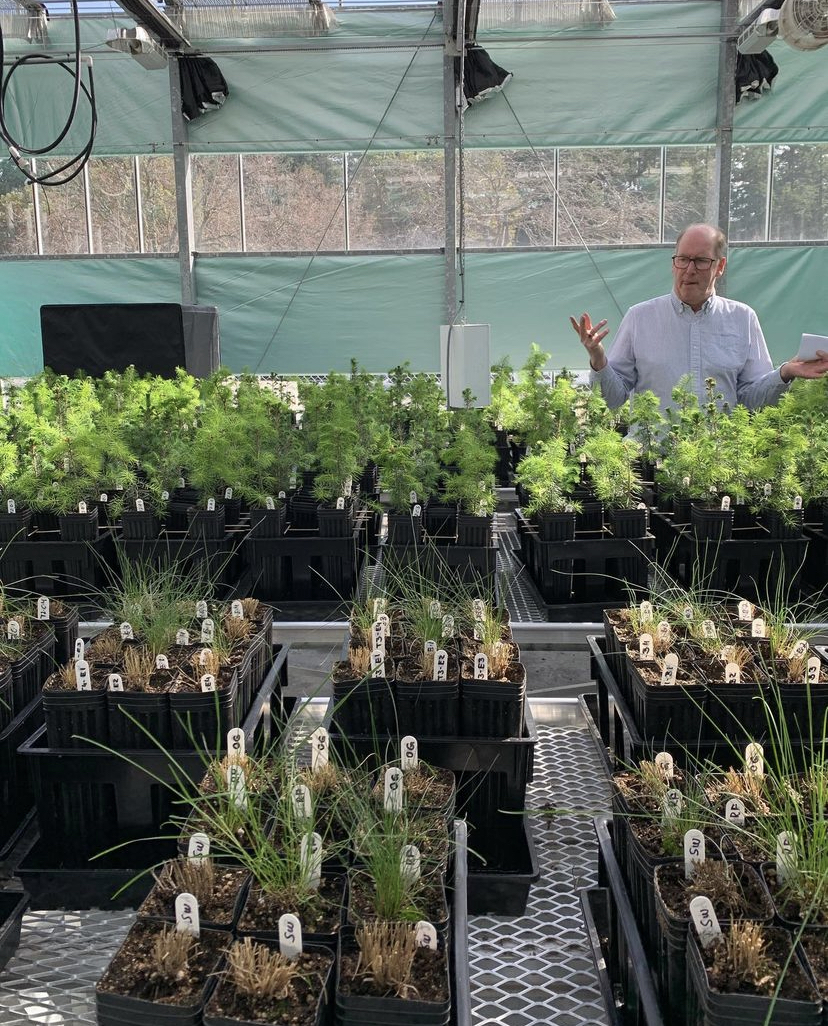
\includegraphics[width=.58\columnwidth]{images/greenhouse.jpg}

\bigskip
\sffamily\lite\fontsize{10}{10}\selectfont\raggedright 
\emph{Above: Dr. Patrick von Aderkas conducted a tour of the Bev Glover Greenhouse for members of the Horticulture Club on March 2nd, exhibiting some of the best the plants the hothouse has to offer.}
\sffamily\lite\fontsize{8}{8}\selectfont\raggedright 
\quoted{(continued on Page 2)}


\end{tabular}

\clearpage

%%%%%%%%%%%%%%%%%%%%%%%%%%%%%%%%%%%%%%%%%%%%%%%%%%%%%%%%%%%%%%%%%%%%%%%%
% Page 2

\noindent\begin{tabular}{@{}
                         p{.38\columnwidth}%		blurb
		         @{\hspace{.04\columnwidth}}% 	gap
		         p{.58\columnwidth}%		quotes
		         @{}%			implicit margin
}

% Left column
\sffamily\lite\fontsize{16}{18}\selectfont\raggedright 
\small\rightskip=0pt
\subsection*{\sffamily Event Recap: Plant Swap!}
The Horticulture Club's first plant swap took place on March 9th in the Student Union Building. Club members were encouraged to bring any plant-related items they had, including soil, pots, and fertilizer. During the event, a game of 'white elephant' was played, and many tomato and onion plants were given away. The turnout was excellent, and the opportunity to share extra plants, tools, and horticultural advice made the event a success.
\par\bigskip
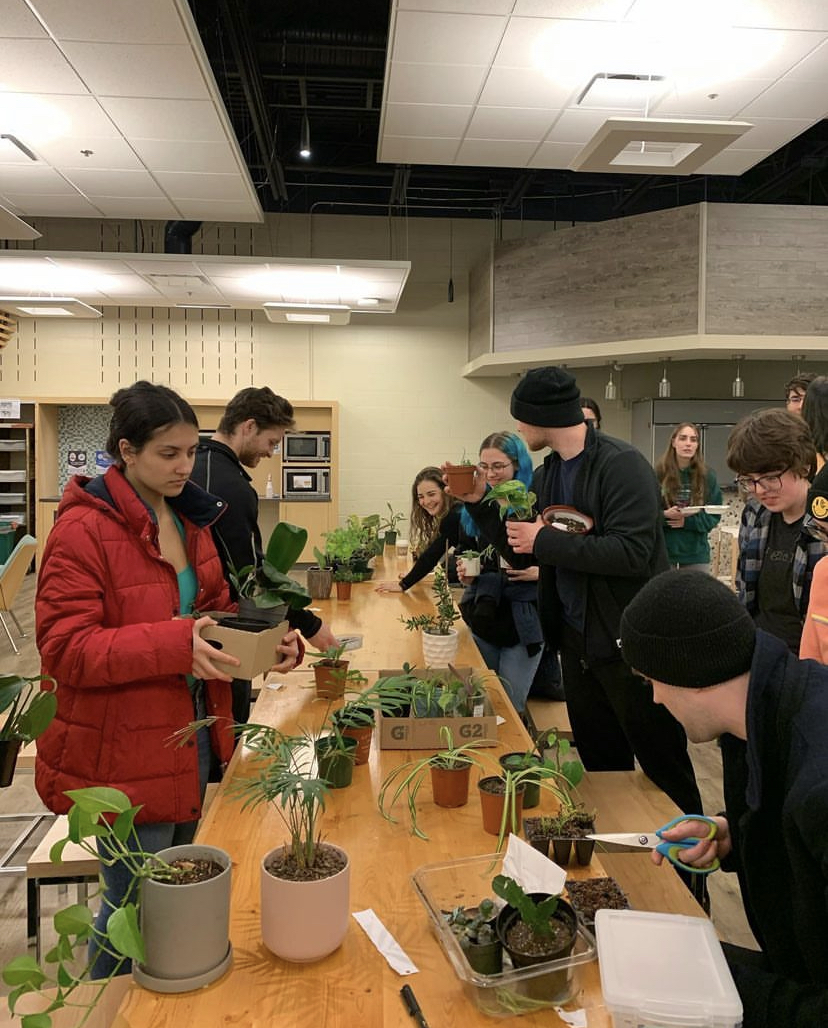
\includegraphics[width=6.8cm]{images/swap.jpg}
\par\bigskip
\emph{Above: Members meet in the Student Union Building to swap plants, give away propagules, and share plant care-taking tips.}
\vfill

% Right column
&\large
\lettrine[lines=3]{}{Continued}: The Bev Glover Greenhouse Facility, named after a Biology lab instructor who passed away in 2001, and was built that same year. The facility contains six climate-controlled greenhouses, which are visible from ring road and hug the west side of Parking Lot 1. \linebreak\
\par\medskip
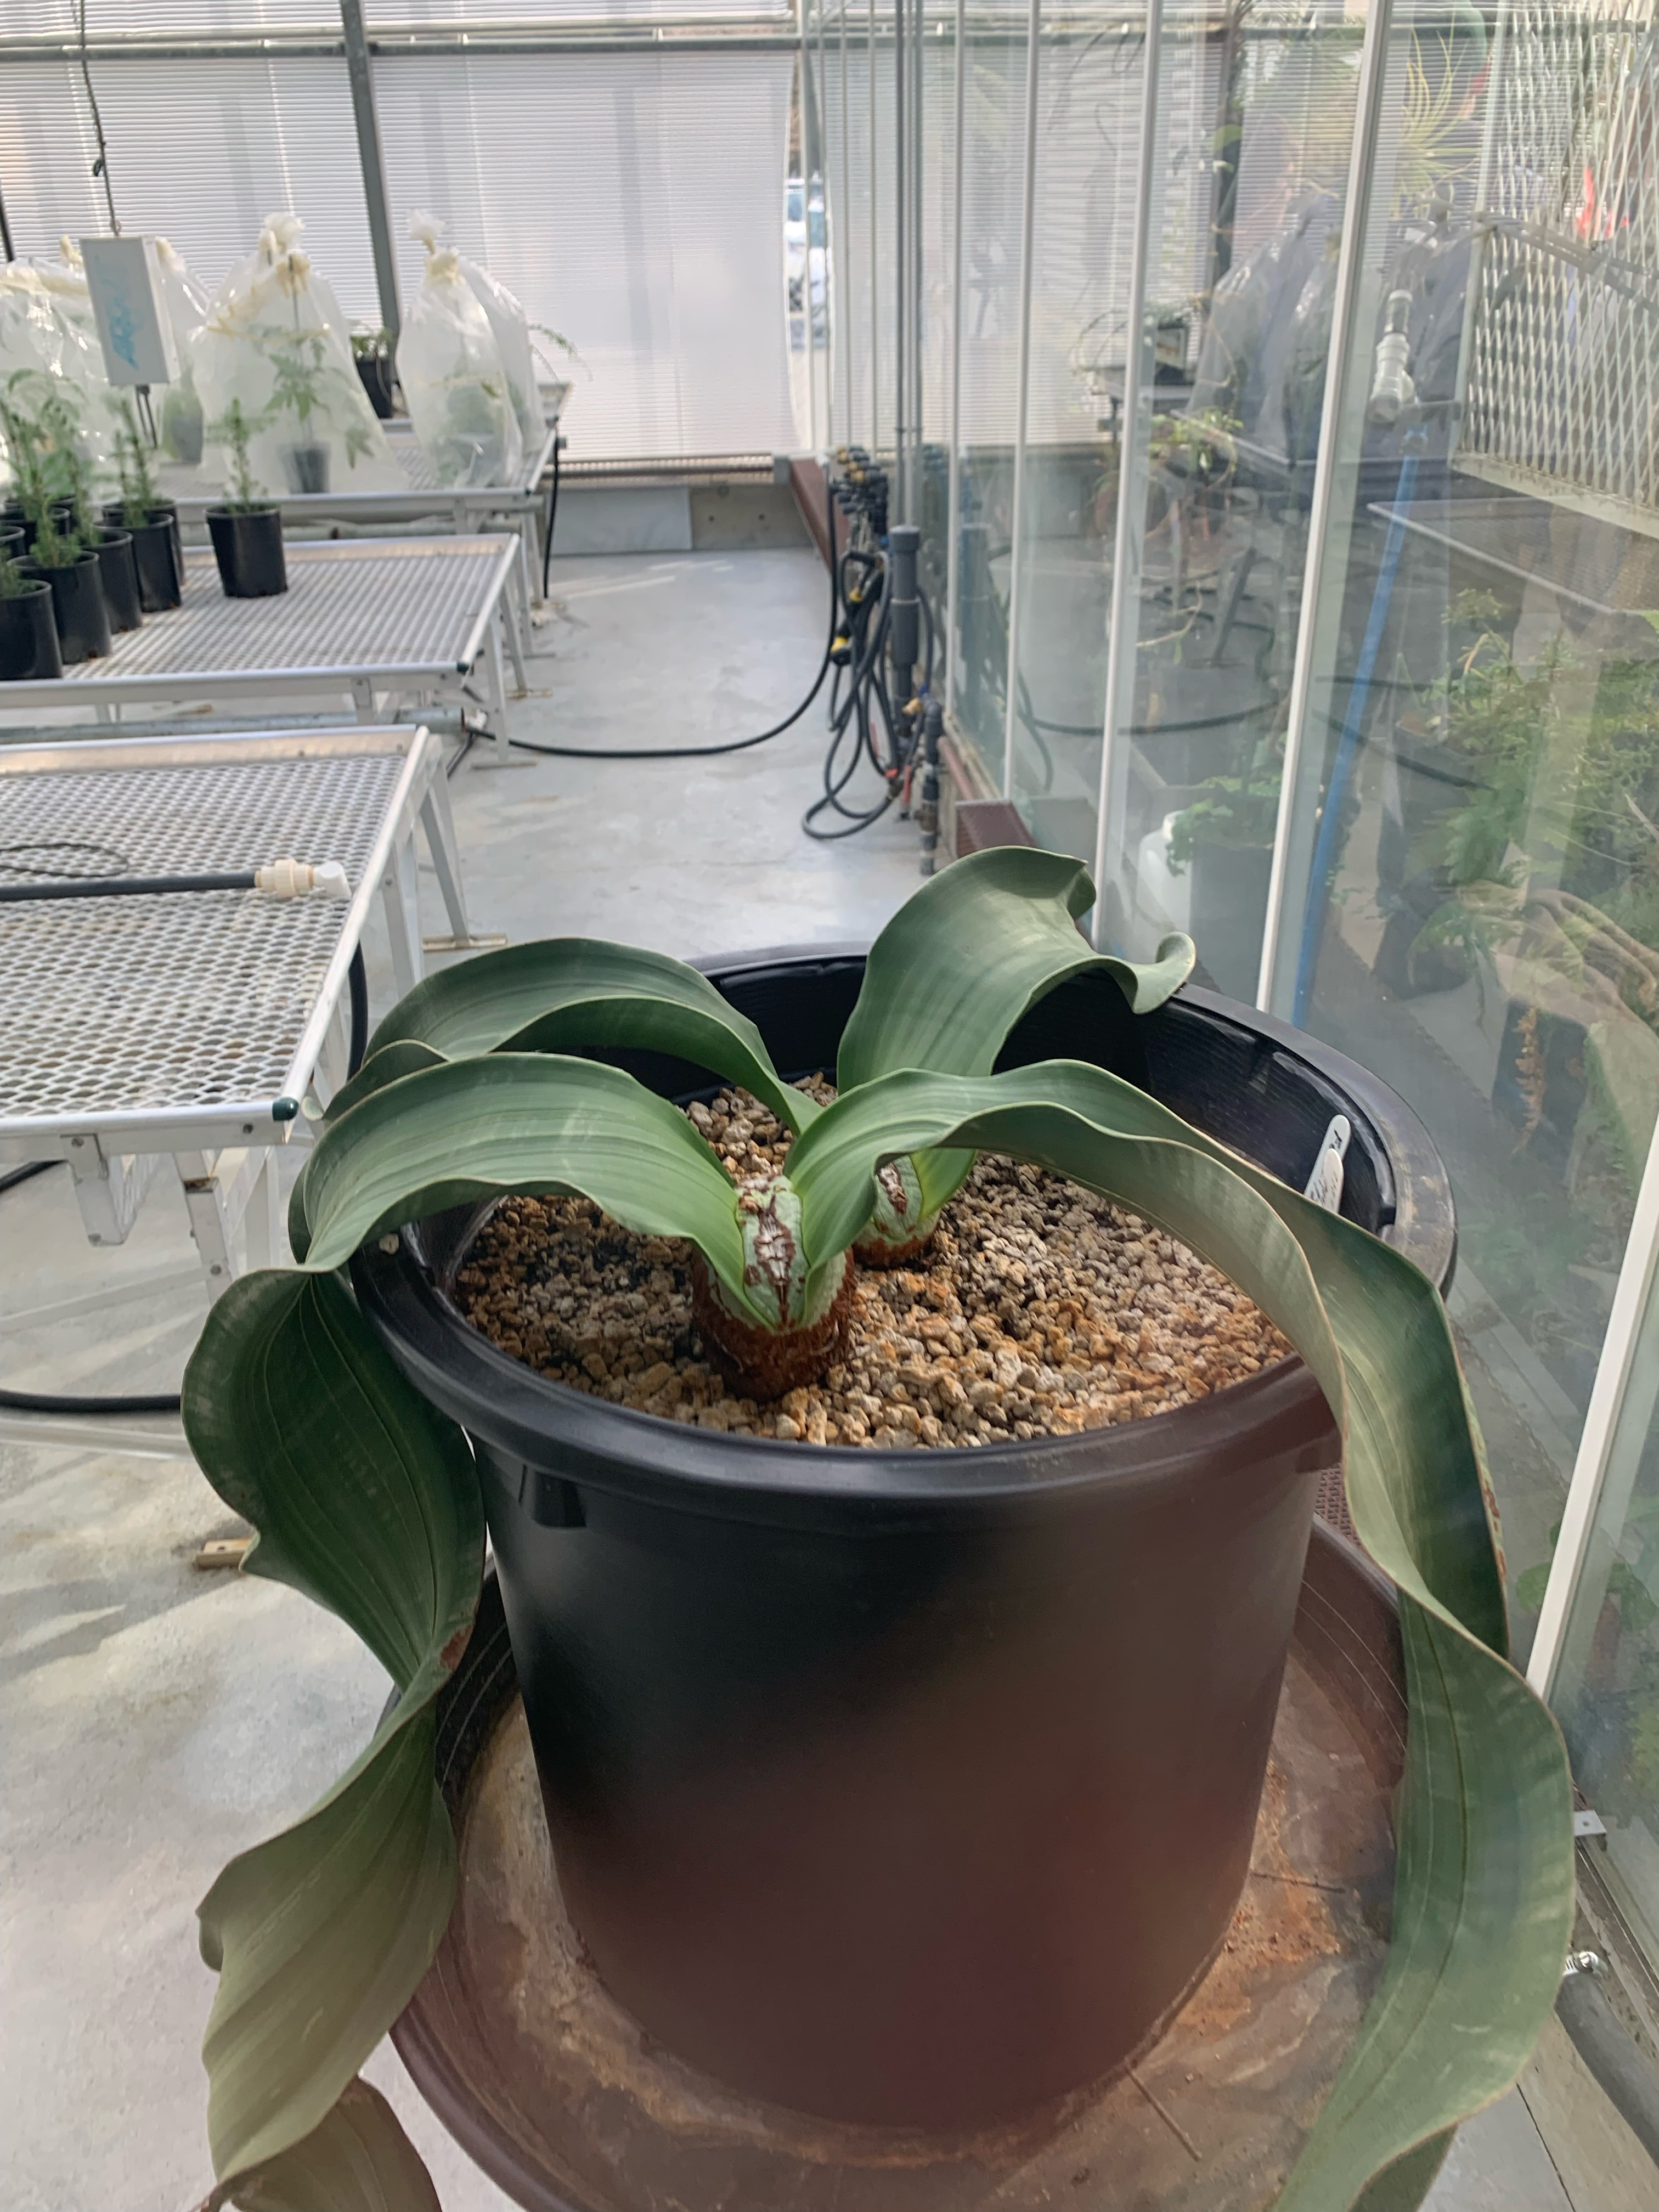
\includegraphics[width=5cm]{images/welwitschia.jpeg}\hfill
\includegraphics[width=5cm]{images/davallia.jpeg}\hfill
\par\bigskip
\includegraphics[width=10.40cm]{images/sundew.jpeg}\hfill
\sffamily\lite\fontsize{10}{10}\selectfont\raggedright 
\par\bigskip
\emph{Above (left to right): \emph{Welwitschia mirabilis}, \emph{Davallia trichomanoide} and \emph{Drosera capensis} are just a few of the plants grown in UVic's greenhouse facility.}
\vfill
\end{tabular}
\clearpage
\end{document}